\section{Introduction}
\subsubsection{Trigeminal Neuralgia}
Trigeminal neuralgia (TN) is a debilitating facial neuropathic pain syndrome characterized by paroxysmal and shock-like pain in one or more divisions of the trigeminal nerve (The fifth cranial nerve, CN V) branches. TN manifests most commonly as classic (also called idiopathic TN), or secondary to a range of neuropathology, including tumors such as meningiomas \cite{Cheng2008}, trigeminal schwannomas \cite{Miller2008}, and most notably multiple-sclerosis (MS) \cite{Cruccu2009,VanderMeijs2002,Nick2012}. The pathophysiology of classic TN is thought to be vascular compression at the root of the CN V nerve entry zone (NEZ) \cite{Linn2011,Love2001}, although classic TN can also occur without evidence of vascular compression \cite{Lee2014}. While the focus of the study of TN has been primarily the peripheral segments of the trigeminal nerve, we recently compared TN and MS-TN diffusivity differences in four segments of the CN V, including at the level of the pons \cite{Chen2016a}, and confirmed that brainstem CN V diffusivity is altered in MS-TN. Similarly, we demonstrated, using multi-tensor tractography, that altered diffusivity at the level of the pons prognosticates treatment non-response \cite{Hung2017}. It appears therefore that TN is associated with unique peripheral abnormalities and brainstem related central abnormalities. 

Investigation of potential gray and white matter findings in TN has demonstrated that there are key abnormalities in areas important for discrimination and modulation of pain, including the thalamus, basal ganglia, primary somatosensory cortex, primary motor cortex, orbitofrontal cortex, cingulate cortex, and insula \cite{Desouza2013c, Desouza2013}.

The trigeminal sensory system involves both discriminative touch and pain pathways \cite{Henssen2016}.  Pain and discriminitive touch stimuli trigger innervations of the three trigeminal nerve branches (V1, V2, and V3) in the head and face, these primary affrents converge and form the trigeminal root gangion (TRG) (also known as Gasserian, or semilunar ganglion) in the middle cranial fossa. The discriminative touch afferents then course through the cisternal segment of CN V, enter the pons, and synapse onto the primary trigeminal sensory nucleus, after which they project to the contralateral VC thalamus and the S1 cortex. The nociceptive pathway synapses caudally onto the trigeminal spinal nucleus, decussates at the level of the medulla and spinal cord. The pathway merges with the discriminative sensory pathway and ascend as the contralateral trigeminal lemniscus, and also project to the contralateral VC thalamus. The pain pathway also projects to the medial nucleus of the thalamus, after which it courses towards the fibers of the cingulate cortex. 

The tractography and diffusivity parameters of the trigeminal pathways more central to the brainstem have not been studied, primarily due to methodological limitations. However there are important elements associated with diffusivity abnormalities in TN, including the observation that brainstem diffusivity abnormalities prognosticate a non-responder status \cite{Hung2017} and bilateral alterations in trigeminal nerve despite a uniformly unilateral clinical expression of pain \cite{Miller2009}. It is therefore relevant to understand the potential TN related abnormalities in more central components of the trigeminal fibers.  

\subsubsection{Along-the-tract analysis}
White matter tractography is commonly used for anatomical visualization \cite{Chen2011b}, white matter segmentation \cite{Behrens2003a,Johansen-Berg2005}, and structural connectivity analysis \cite{Cao2013,Wiech2014}. This analysis invovles obtaining diffusivity metrics from tractography after converting streamline bundles into a volumetric spatial mask and measurement of the mean metric from all or parts of the masked voxels \cite{Concha2005,Fitzsimmons2009}. However this approach discards the orientation information in the streamlines. The simplest form of spatial masking is to identify voxels where at least one streamline has passed through it, which often results in identifying voxels with minimal streamline pass-throughs. This is potentially problematic when considering that an average 3-Tesla HARDI DWI acquisition has a voxel dimension of 2 to 3 mm \cite{Neher2015,Wilkins2015}. In white matter structures such as CN V as well as other small pathways, the structure diameter may be fairly small (less than 3 mm) and therefore the naive spatial masking approach would result in severe partial volumes that will confound the result. 

For a tractography streamline propagation algorithm to address these limitations, it must involve all or parts of the following stages: 1) subsampling of an initial region for seeding \cite{Basser2002,Cote2012}; 2) identifying a propagation direction, based on previously traversed paths \cite{Malcolm2010,Qazi2009,Tournier2010}; 3) smoothing of the traversed paths for output \cite{Tuch2000d}. It is reasonable to consider these algorithms to be an interpolated subsampling scheme of the DWI volume that takes the diffusion-based orientation into account. Therefore, it would be desirable to directly make use of the tractography streamlines for data measurement. 

Along-the-tract analysis has been investigated by various authors \cite{Colby2012,ODonnell2009,Wang2015,Yeatman2012}. Commonly, the bundles were selectively filtered from global tractography \cite{Wang2015,Yeatman2012}. An spatial representative curve, termed the tract centroid, was determined for the streamlines that consist of the bundle. The centroid was calculated by a variety of distance measures between the points of the streamlines \cite{Garyfallidis2012}, and resampled to a certain number of subpoints. The diffusivity metrics from each streamline points were pooled onto the tract centroid in each individual subjects, and then aggregated at the group level. In this way, diffusivity metrics within a tractography bundle in 3D space would be projected to a 1D centroid for detailed analysis. 

The global tractography approach is limited to major white matter bundles, and unintuitive for anatomy-specific tasks in a clinical environment, where the anatomy of interest is predetermined. A more focused ROI based delineation approach is therefore preferred in these circumstances. We have developed the Selective Automated Group Integrated Tractography (SAGIT) framework \cite{Chen2016} to automate group-wise tractography delineation, which ensures consistent region-of-interest (ROI) projection, tractography seeding sampling scheme, and tractography parameter tuning. This technique permits tracts to be merged into a template space using non-linear deformations. A centroid can be directly defined on the merged tractography bundle, and the diffusivity metrics from multiple subjects can be pooled onto the centroid directly. The extact diffusivity data can then be analyzed by machine learning.

\subsubsection{Gaussian Process}
The breakthrough results of deep convolutional neural networks in computer vision \cite{Krizhevsky2012} have sparked the interest of deploying similar systems for medical imaging diagnosis \cite{Greenspan2016}. However, one disadvantage of deep neural networks is in its inability to quantify uncertainty and provide interpretable models. Model interpretability is a fundamental requirement for machine learning in medicine, and therefore there is renewed interest in bayesian-based models like Gaussian Process (GP) \cite{gal2016dropout}.

The streamline measurements resembles time-series data, in that it exhibits positional dependency between measurements. Unlike a time-series however, the measurements represent physical locations along a pathway, thus exhibiting bi-directional dependency. Posing the study as a supervised machine learning problem, the feature vector would be an N-dimensional vector representing N measures at each division. The GP classifier models the feature vector as a latent GP model, before squashing it to produce a logistic output. Therefore the GP model is able to take the positional dependency of the measurements into account, and is well suited for streamline-based classification.

Gaussian Process is defined \cite{rasmussen2006gaussian} as a collection of random variables, any finite number of which have a joint Gaussian distribution. 
It is a distribution that is defined by a mean function $m(x)$ and covariance function $k(x,x') $ where
\begin{equation}
	\begin{split}
		m(x) &= \mathbb{E}[f(x)], \\
		k(x,x') &= \mathbb{E}[(f(x)-m(x))(f(x')-m(x'))],
	\end{split}
\end{equation}
and the Gaussain processed is defined as
\begin{equation}
f(x) \sim GP(m(x), k(x, x')) 
\end{equation}

The covariance function is also called the kernel function. The radial-basis function kernel (RBF kernel) is widely used in machine learning tasks. GP has previously been explored in neuroimaging for tractography clustering \cite{Wassermann2010} and it is particularly well suited for continuous data streams, such as tractography streamlines.

In all previous TN studies, placements of measurement region-of-interests in the CN V were pre-planned and manually placed by researchers. Manual tractography generation with manual ROI placements was a roadblock in performing more in-depth group-wise tractography examination of the trigeminal pathways. We had developed and validated the SAGIT tractography framework to allow automated group tractography \cite{Chen2016}. We further expand, in the current study to A) analyze the CN V differences between TN and healthy controls across the entire peripheral segment of the nerve using along-the-track and machine-learning methods to auto-discover key regions-of-interest; B) extend the examined regions to include trigeminopontothalamic (TPT) and thalamocortical (S1) white matter pathways as part of the trigeminal sensory pathways.

\section{Methods}

The overall processing steps are a) generation of merged tractography bundle of each trigeminal pathway; b) definition of centroids that spatially represent each pathway, and pooling the diffusivity data from streamlines onto the centroid; and c) scroll a moving window along the centroid positions, and train a GP classifier at each step, the windows with the best accuracy is then determined. The details are as follows.

\begin{figure}[ht]
\centering
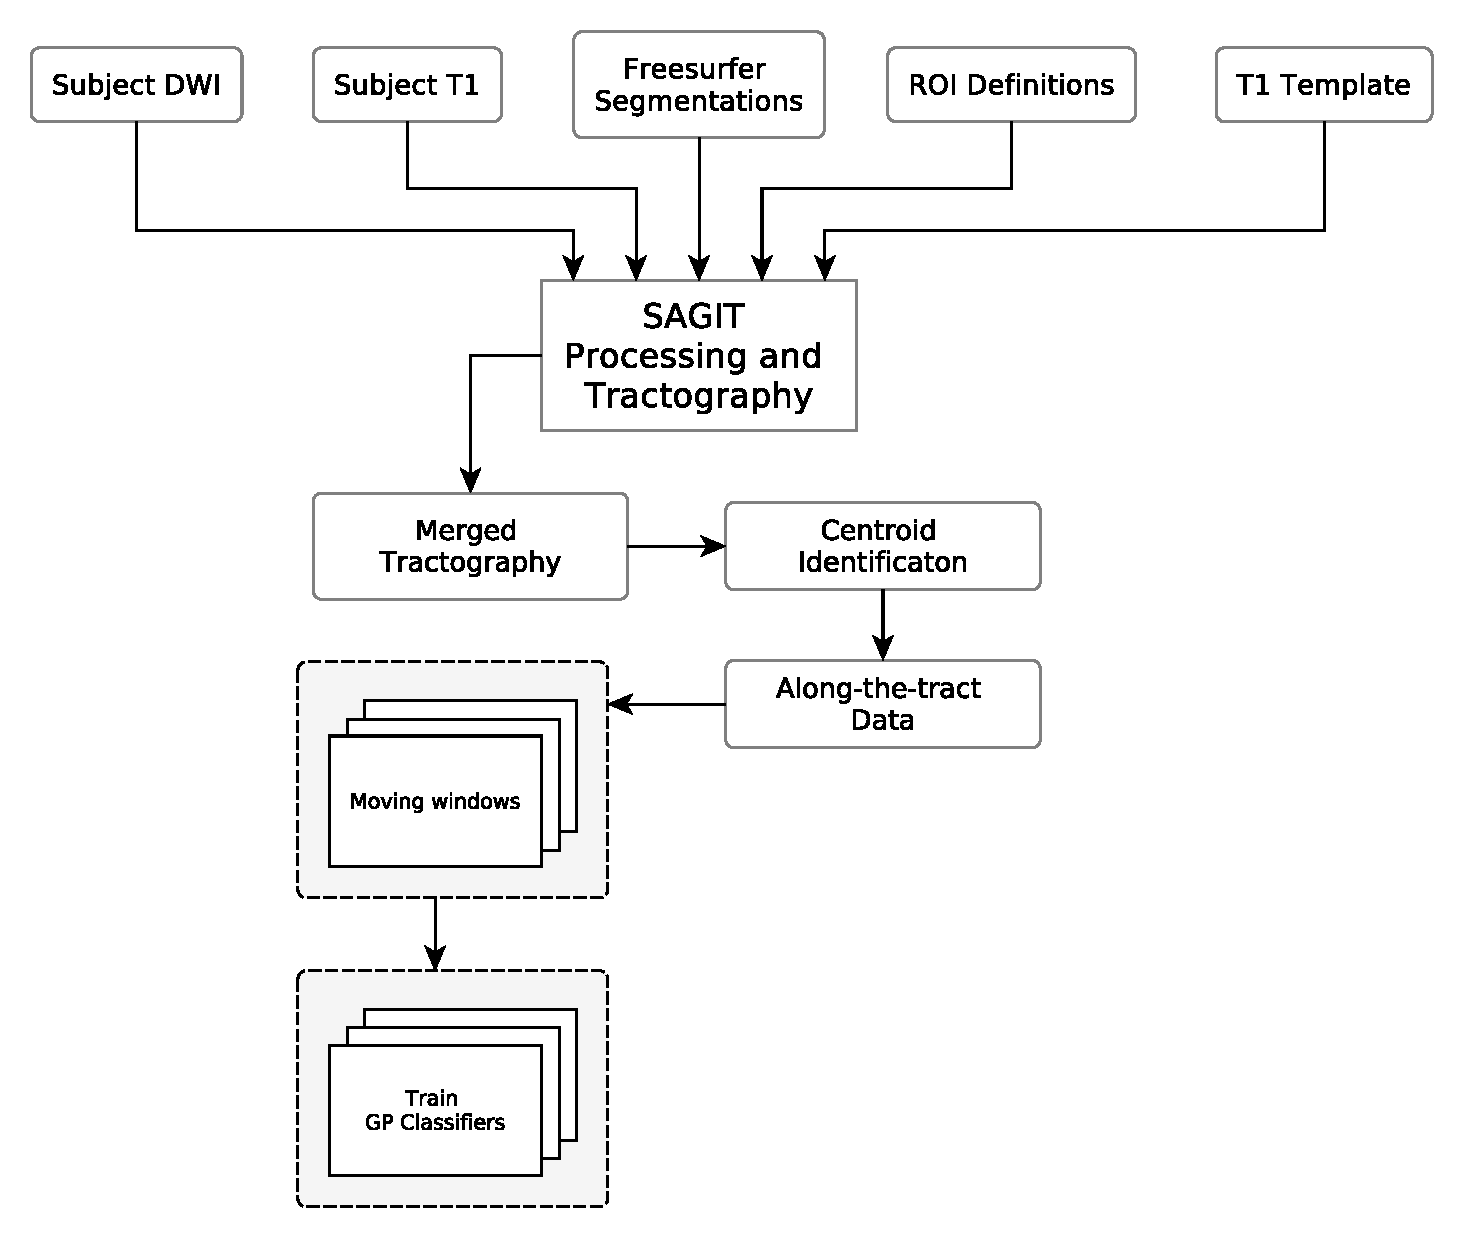
\includegraphics[width=\linewidth]{figure-method.pdf}
\caption{Diagram of the overall processing steps. The details of SAGIT processing steps can be found in \protect\cite{Chen2016}. Details of the centroid identification can be found in Figure \ref{fig:GPfigure-method-centroid}. The details for machine learning process can be found in Figure \ref{fig:GPfigure-gp-train}. }
\label{fig:GPMethods}
\end{figure}

\subsubsection{Acquisitions}
We studied 36 TN subjects with classic TN (28 females, 8 males; age 60.1$\pm$16.0 years; right sided pain), and 36 healthy controls (28 females, 8 males, age 42.7$\pm$12.0 years).  All TN subjects underwent non-invasive Gamma Knife radiosurgery, with imaging prior and six months post treatment. MRI acquisitions including T1 fast-spoiled gradient echo (FSPGR) and diffusion weighted image (DWI) acquisitions. 
T1 scans were acquired with 1mm slice thickness, in-plane resolution of 0.9375x0.9375 mm, with slice spacing = 1 mm, TE = 5.052 ms, TR = 11.956 ms, flip angle = $20^\circ$, FOV = 240 mm, and matrix = 256x256. 
DWI scans were acquired with 1 B0 scan, 60 gradient directions, 3 mm slice thickness and an in-plane resolution of 0.9375x0.9375 mm, where b0 = 1000 s/$mm^2$, TE = 88.6 ms, TR = 17000 ms, flip angle = $90^\circ$, field of view (FOV) = 120 mm, and matrix = 128x128.

\subsubsection{Preprocessing}
DWI images were motion/eddy-current corrected, with appropriate correction applied to the b-matrix \cite{Leemans2009}. ROI for tractography seeding were manually created on a normalized template brain from 42 healthy brains \cite{Chen2016}. The normalized brain template was created using Anatomical Normalization Tools \cite{Avants2010,Avants2011}. We deployed selective automatic group integrated tractography (SAGIT) framework \cite{Chen2016} to automate preprocessing, registration, and tract generation. The SAGIT processing steps are as follows: T1 anatomical images were processed using FreeSurfer \cite{Fischl2004} for cortical and subcortical segmentations. The T1 images for all the subjects were registered to the template using symmetric diffeomorphic registration (SDR) \cite{Avants2008b}. Each individual DWI was registered to their T1 image with SDR, using mean DWI image for DWI-T1 co-registration. Freesurfer segmentation maps were first affine transformed from the Freesurfer space to the T1 space using FMRIB's Linear Image Registration Tool (FLIRT) \cite{Jenkinson2001,Jenkinson2002}, and then transformed using SDR transforms to the individual DWI space for selective ROI generation with SAGIT.

\subsubsection{Tractography}
ROIs were defined on the template image to delineate the following bilateral structures: 1) CN V (specifications: ROI placed at cistern nerve root; excludes regions of cerebellum grey matter and pontine cerebellar peduncles); 2) trigeminothalamic pontine decussation (TPT) (ROIs placed at trigeminal nucleus (TGN); the fibers must traverse pontine decussation towards contralateral VC thalamus; pathway must exclude ipsilateral thalamus, cerebellar grey matter, pons, and contra-lateral S1 ); 3) thalamocortical S1 pathway (ROIs placed at VC thalamus; pathway must traverse the ipsilateral S1 white-matter boundary and exclude the brainstem).  

We used constrained spherical deconvolutional tractography (CST) \cite{Tournier2012b} to delineate the three defined anatomical regions. Deterministic and probabilistic streamline algorithms were used to delineate different regions, based on findings in the SAGIT study \cite{Chen2016}. Deterministic CST was applied to delineate CN V and S1 anatomy, while probabilistic (iFOD2) CST \cite{Jeurissen2011b,Tournier2010} was applied to delineate TPT anatomy. The parameters for each were as follows: Deterministic CST was performed with step size = 0.3 mm, angle threshold = $45^\circ$, streamline count = 200, minimal length = 5 mm, initial cut-off = 0.1, cut-off = 0.1, and with 4th-order Runge-Kutta integration. Probabilistic tractography for S1 projection was performed with step size = 5mm, angle threshold = $45^\circ$, streamline count = 300, max number of stream generation = 1 million, minimal length = 10 mm, maximum length = 80 mm, initial cut-off = 0.15, cut-off = 0.15. Probabilistic tractography for TPT project was performed with step size = 1 mm, and streamline count = 2000, and maximal length = 60 mm. Tractography was first performed in the native DWI space for each subject.  FA, AD, RD, MD, and GFA were embedded into the native tractography models by sampling the corresponding images maps using the points of the tractography geometry with tri-linear interpolation.

\subsubsection{Merged Tractography}
All tractography delineations of the same anatomy across all the subjects and groups were merged into a single tractography file for analysis. We have previously created a software library\footnote{https://github.com/sinkpoint/fascicle} to facilitate this process. Detailed steps are as follows: The individual tract files were converted into a SQLite relational database \cite{owens2010sqlite}, and  all points were exported and transformed by applying the subject DWI to T1, and T1 to template transforms using ANTS' applyTransformToPoints command \cite{Avants2009}. The transformed points were then imported back into the  database, and a new template-space tractography model is exported using the transformed point-set, with all its original scalars and subject/group associations preserved. Finally, all template-space tractography models across all the subjects are merged into a single file. 
The merged tract was post-processed in 3D Slicer to remove anatomically erroneous streamlines. These include remnant CN V streamlines that stray into the cerebellar peduncles or other non-TGN regions, and streamlines that are perpendicular to the nerve in the cisternal space that appear to be partial delineation of vessels or noise. TPT streamlines that did not decussate at the level of the pons, as well as fibers that stray into the contralateral TGN were removed. S1 streamlines that stray medially towards other regions such as the corpus callosum were also removed.

\subsubsection{Along-the-tract Analysis}
For the purpose of quantifying the trigeminal pathways, a centroid was defined for the merged tractography of each pathway (Figure \ref{fig:GPfigure-method-centroid}). The centroids were defined as the average curve that best fit the tract bundles and were in template space. CN V centroids were manually defined using 3 control points. A Catmull-Rom spline \cite{DeRose1988} was then defined from these control points using the VTK software library \cite{Schroeder2005}. The spline was then resampled into 30 subpoints. TPT and S1 centroids were defined using QuickBundles \cite{Garyfallidis2012} with distance threshold of 30. Nearest-neighbor point assignment was used to cluster the points of the merged tract model to the centroid subpoints, to obtain the corresponding 30 divisions along each centroid. Diffusion metrics from the tractography points were averaged for each of the divisions for each subject. 

\begin{figure}[ht]
\centering
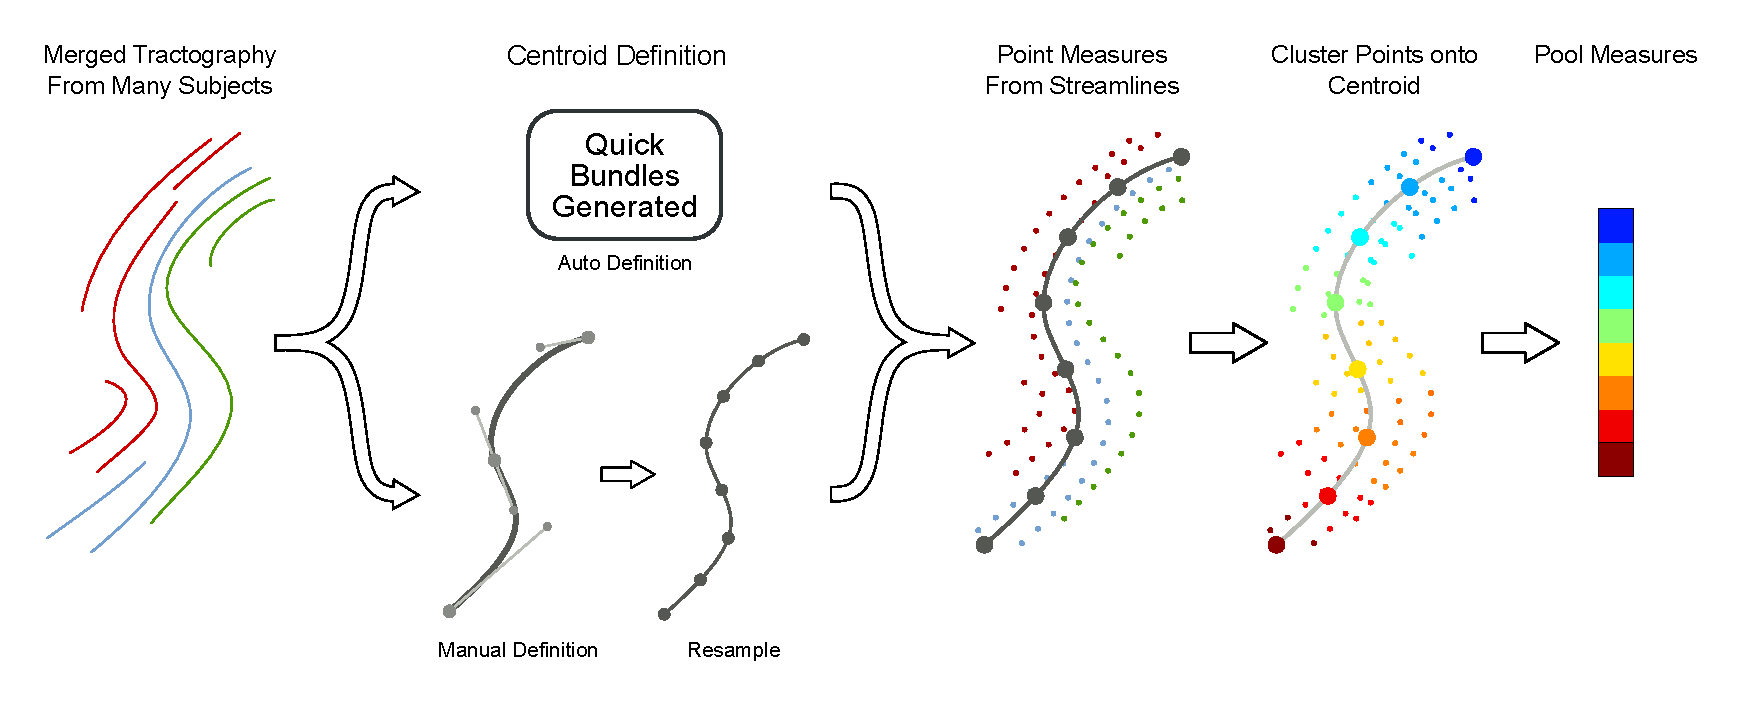
\includegraphics[width=\linewidth]{figure-path-analysis.pdf}
\caption{Diagram for the along-the-tract data processing.
Process starts with 2 specific goals: 1) Derive the spatial structure that best represent the merged streamlines, 2) Deriving sub-regional tissue information from these. A) First the best-fit curve is obtained to represent the collective streamlines, which is defined as the centroid. B) In areas where this can be automated, Quickbundles was used. For the CN V, the centroid was defined manually given the unpredictability of the lengths of streamlines. C) Representative drawing of the centroid onto the streamline points, representing the collective spatial information. The centroid is resampled to 30 subpoints. D) To derive tissue information, a nearest neighbor algorithm was used to assign streamline points to form 30 divisions. E) The average diffusivity metrics was pooled for each of the 36 subjects at each division. The colours represent the spatial position of each of the 30 divisions, and the streamline points that were assigned to each particular division. The data was then used for machine learning pipeline (see Figure \ref{fig:GPfigure-gp-train}).
}
\label{fig:GPfigure-method-centroid}
\end{figure}

\subsubsection{Gaussian Process Classification}

Diffusivity metrics of affected (right side) and unaffected CN V, TPT, and S1 pathways were independently compared with those of controls, where control metrics were the average of both left and right sides. The affected and unaffected sides in TN subjects were also compared with each other. 
Age was regressed out by using the residuals of the linear regression model from the controls group. The diffusion values were subsequently normalized to zero-mean with ranges $[-1, 1]$ for model training. 
Gaussian Process (GP) classification was performed to identify windows that resulted in the highest classification accuracies. Multiple moving windows of length between 5 to 30 were used to scroll through the centroid positions, and a Gaussian Process model was trained for each window (Figure \ref{fig:GPfigure-gp-train}). The machine learning process was performed using Scikit-learn machine learning software framework.
For each window, the subjects were split into train and validation sets using stratified 10-fold cross-validation, and a separate GP classifier was trained for each fold. GP models were initiated with Matern kernel (length scale = 1). The validation set was used to measure prediction accuracy, and the mean accuracy of the 10-fold cross-validation was used to assess the windows. Classification accuracy greater than 70\% were accepted, and the window with the greatest accuracy was then determined. 

\begin{figure}[ht]
\centering
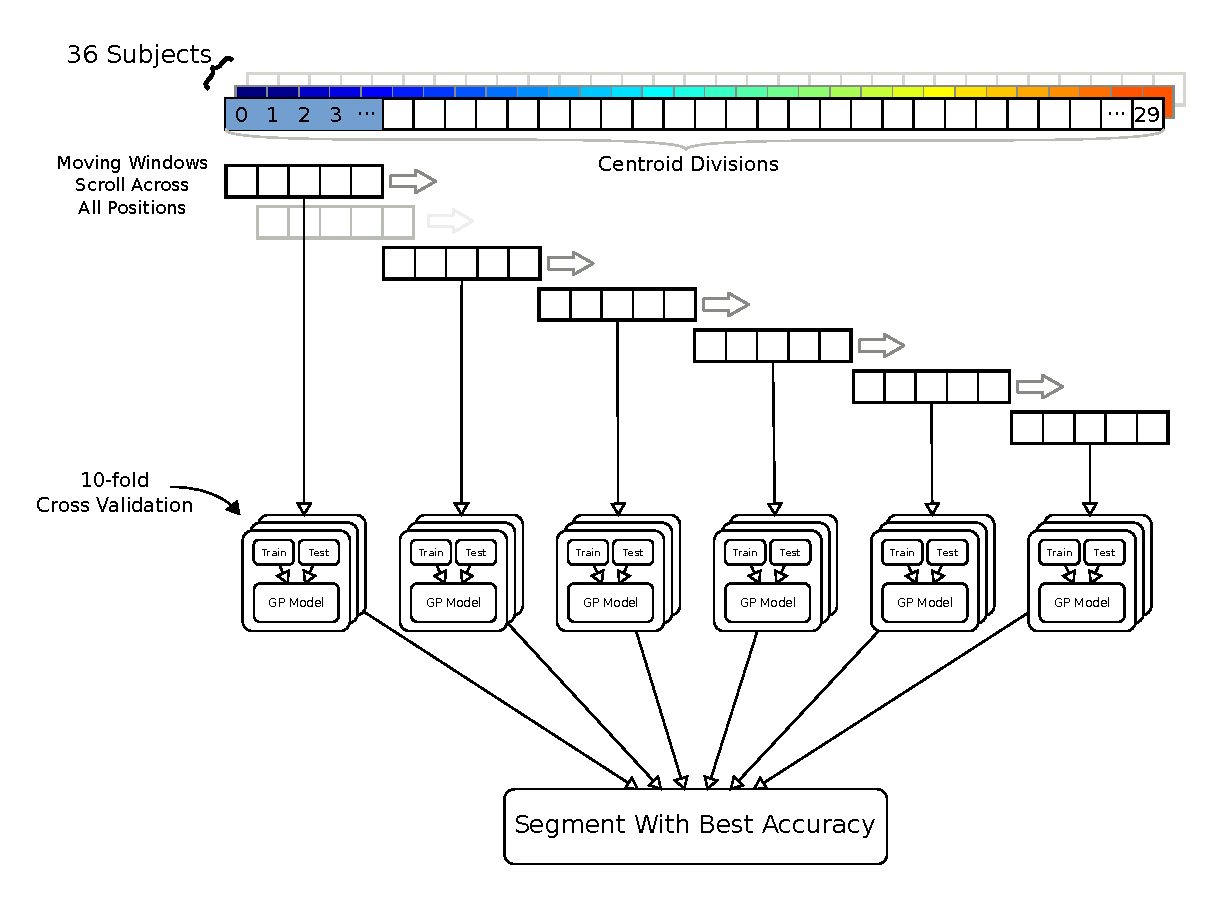
\includegraphics[width=\linewidth]{figure-GP-training.pdf}
\caption{Diagram for generating the best performing classifier for a particular window size. The data was derived from Figure \ref{fig:GPfigure-method-centroid}, where the top bar represents data from each centroid division, and each position represents the anatomical region of the trigeminal pathways within it. Each window was used to generate 10 GP models with 10-fold cross-validation, an average accuracy was determined at each window position. Finally the window position with the best accuracy was selected. The same process is repeated on every diffusivity metric, and for all window sizes ranging from 5 to 30. }
\label{fig:GPfigure-gp-train}
\end{figure}

\subsection{Results}
\subsubsection{Anatomical Delineations}
The findings in each of the three trigeminal areas are as follows: Merged CN V delineations show anatomical consistency from their position in the cisternal segment of the nerve and extending into the ipsilateral TGN. Changes in FA along the streamlines demonstrate clear step-wise increase at the interface between cistern and pontine segments, which is consistent with observations in single subjects. The FA metric of each point was sampled from the native DWI space of each subject, prior to the template space deformations. Therefore the sharp transition in FA in this anatomical landmark suggesting good agreement in the SAGIT anatomical registration (Figure \ref{fig:GPfigure1}). The CN V centroid curve length was determined as 38.91 mm, with the length of each subdivision being 1.3 mm.
The TPT projections from the TGN to the ipsilateral VC thalamus region showed distinct bundles of decussating pathways in both left and right projections. The resulting pathways were not symmetrical, where the right TPT pathway appears to divert around the left (Figure \ref{fig:GPfigure2}).
S1 streamlines reliably extended into the face region of the S1 cortex (Figure \ref{fig:GPfigure3}). The S1 centroid curve length was calculated to 62.1 mm and sub-division length was 2.07 mm.

\begin{figure}[ht]
\centering
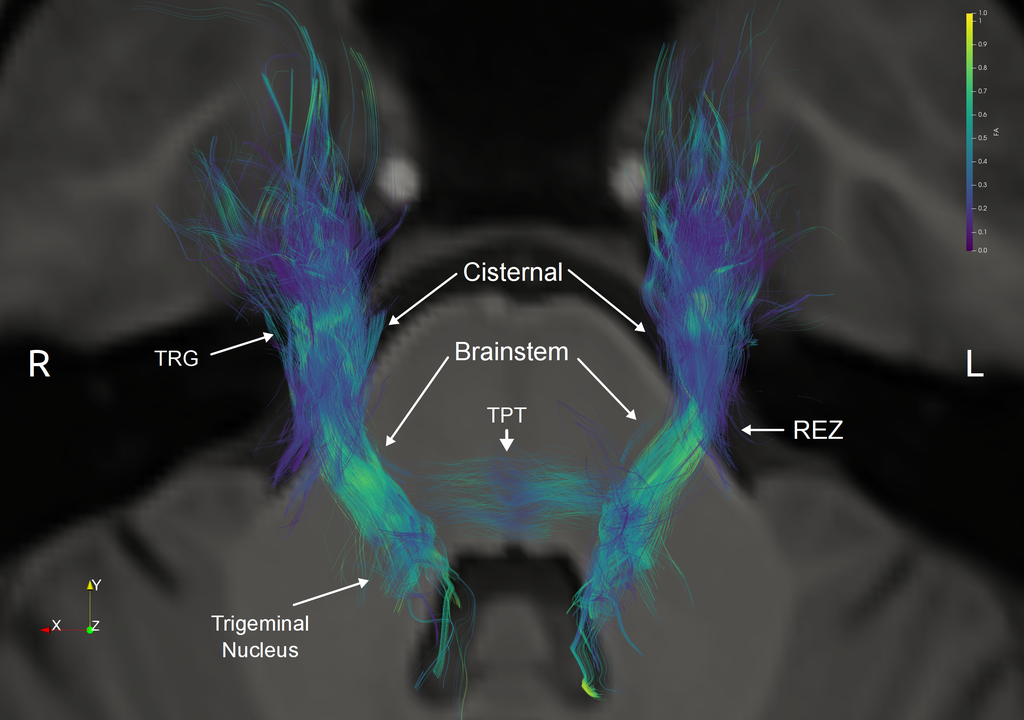
\includegraphics[width=\linewidth]{cnv-inferior-view-annotated.png}
\caption{Merged CN V reconstruction of 36 subjects, with the colour scale depicting FA values derived from raw streamlines, prior to the generation of centroids (see Figure \ref{fig:GPfigure-method-centroid} A). The expected increase in FA as the fibers enter the brainstem can be visualized, and denotes good registration between subjects. }
\label{fig:GPfigure1}
\end{figure}

\begin{figure}[ht]
\centering
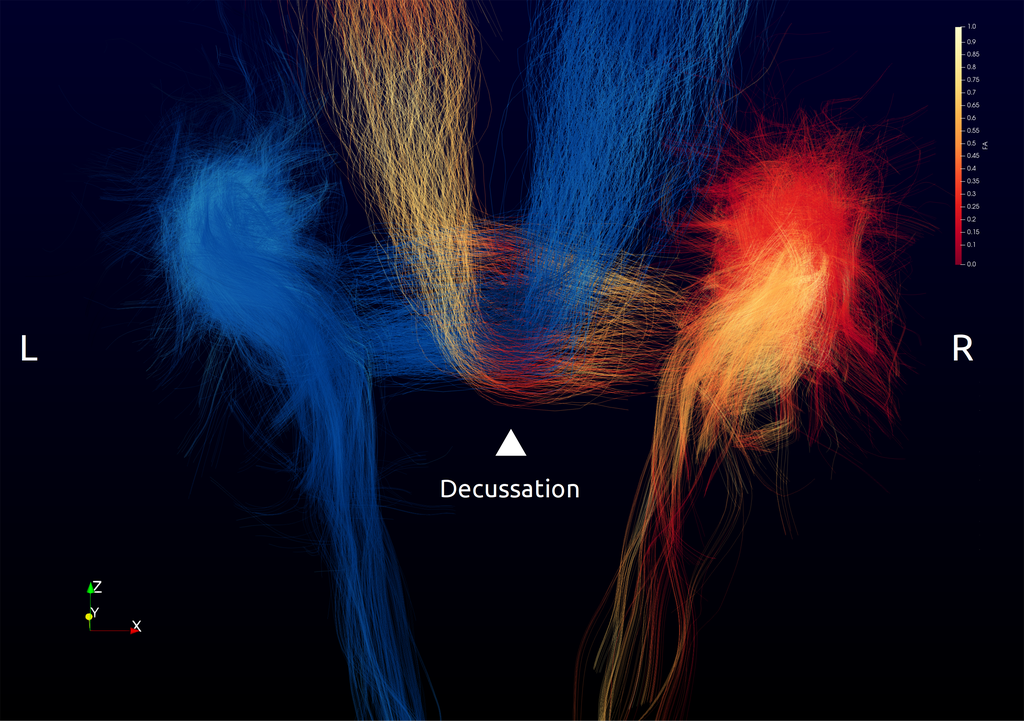
\includegraphics[width=\linewidth]{view-decussation.png}
\caption{Focused view of the TPT and its decussation, prior to the generation of centroids (see Figure \ref{fig:GPfigure-method-centroid} A). Colours were chosen arbitrarily to denote left and right pathways, however the colour intensity represents FA values as depicted by FA scale, top right corner. Red: Right TPT; Blue: Left TPT. Note the Right TPT appears to divert around the left TPT bundle. }
\label{fig:GPfigure2}
\end{figure}

\begin{figure}[ht]
\centering
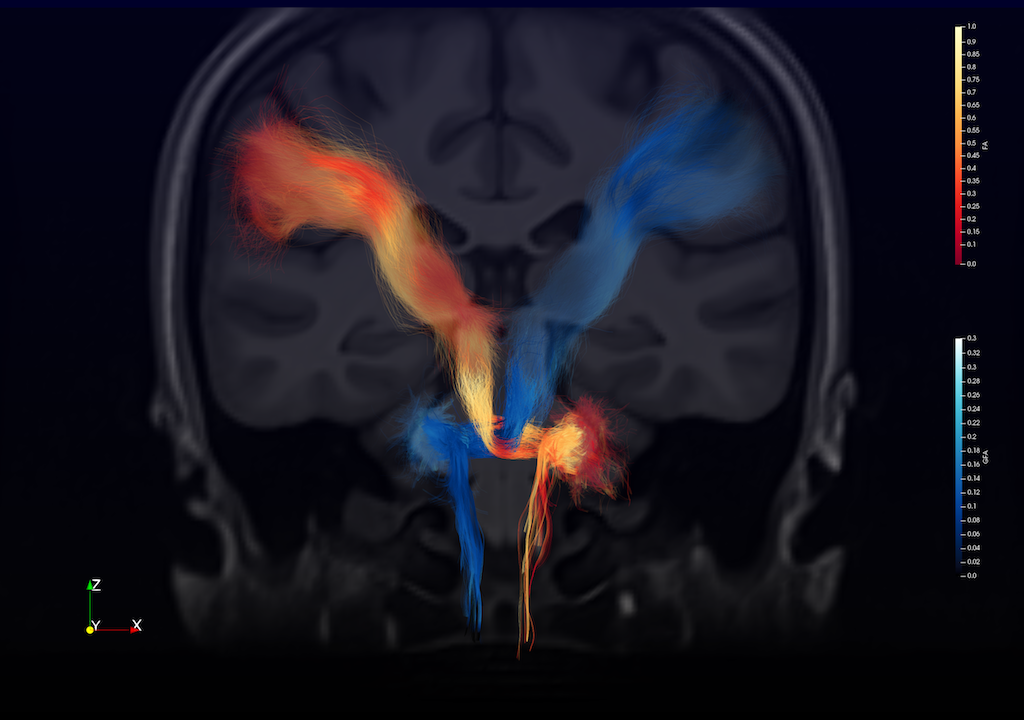
\includegraphics[width=\linewidth]{view-left-right.png}
\caption{Visual representation of the course of the trigeminal pathway from its cisternal component to the face area of the sensory S1 cortex. Images obtained prior to the generation of centroids (see Figure \ref{fig:GPfigure-method-centroid} A). FA is depicted by the colour intensities (Red: right side; Blue: left side). The trigeminal nerves, including the cisternal segments are seen in a coronal perspective (CN V), following which two pathways can be seen. The first pathway appears to head into the spine, while the second pathway consists of the TPT. Following the decussation, the fibers proceed to the area of the sensory thalamus and from there to the cortical sensory area S1.}
\label{fig:GPfigure3}
\end{figure}

\subsubsection{Diffusivity Differences}
\paragraph{CN V}
The classifier distinguished bilateral trigeminal nerves (affected and unaffected) from controls as well as affected trigeminal nerve from unaffected nerves. Both sides were distinguished from controls with classifiers that achieved near 80\% accuracy (Figure \ref{fig:GPfigure4}). 
Classifiers on the right (affected) side had accuracies ranging from 76\% (GFA) to 86\% (FA). The left (unaffected) classifiers achieved accuracy ranging from 79\% (MD) to 81\% (FA). The right side showed greater overlap of segment ranges between positions 14--24, which corresponds to the region of the cistern/ganglion; while the left side showed segments that covered the entire the nerve, and extended to cover position 0--4, within the substance of the trigeminal fibers in the brainstem. Overall, the windows of the right side classifiers extend further into the distal subdivisions, into the cistern and the area of the ganglion, while the left side extended more into the brainstem. FA classifier consistently achieved the highest accuracy in both sides, with right side at position 17--23 (cistern/ganglion) and left FA at 2--16 (brainstem/cistern).
The FA classifier achieved 75\% accuracy in differentiating affected versus unaffected nerves, where its segments ranged from 11 to 19, which was the cisternal segment. The GFA classifier achieved 70\% accuracy in region 9--12. Demonstrating that affected-unaffected diffusivity differences were found primarily in the cistern/REZ (Table \ref{table:GP}).

\begin{figure}[p]
\centering
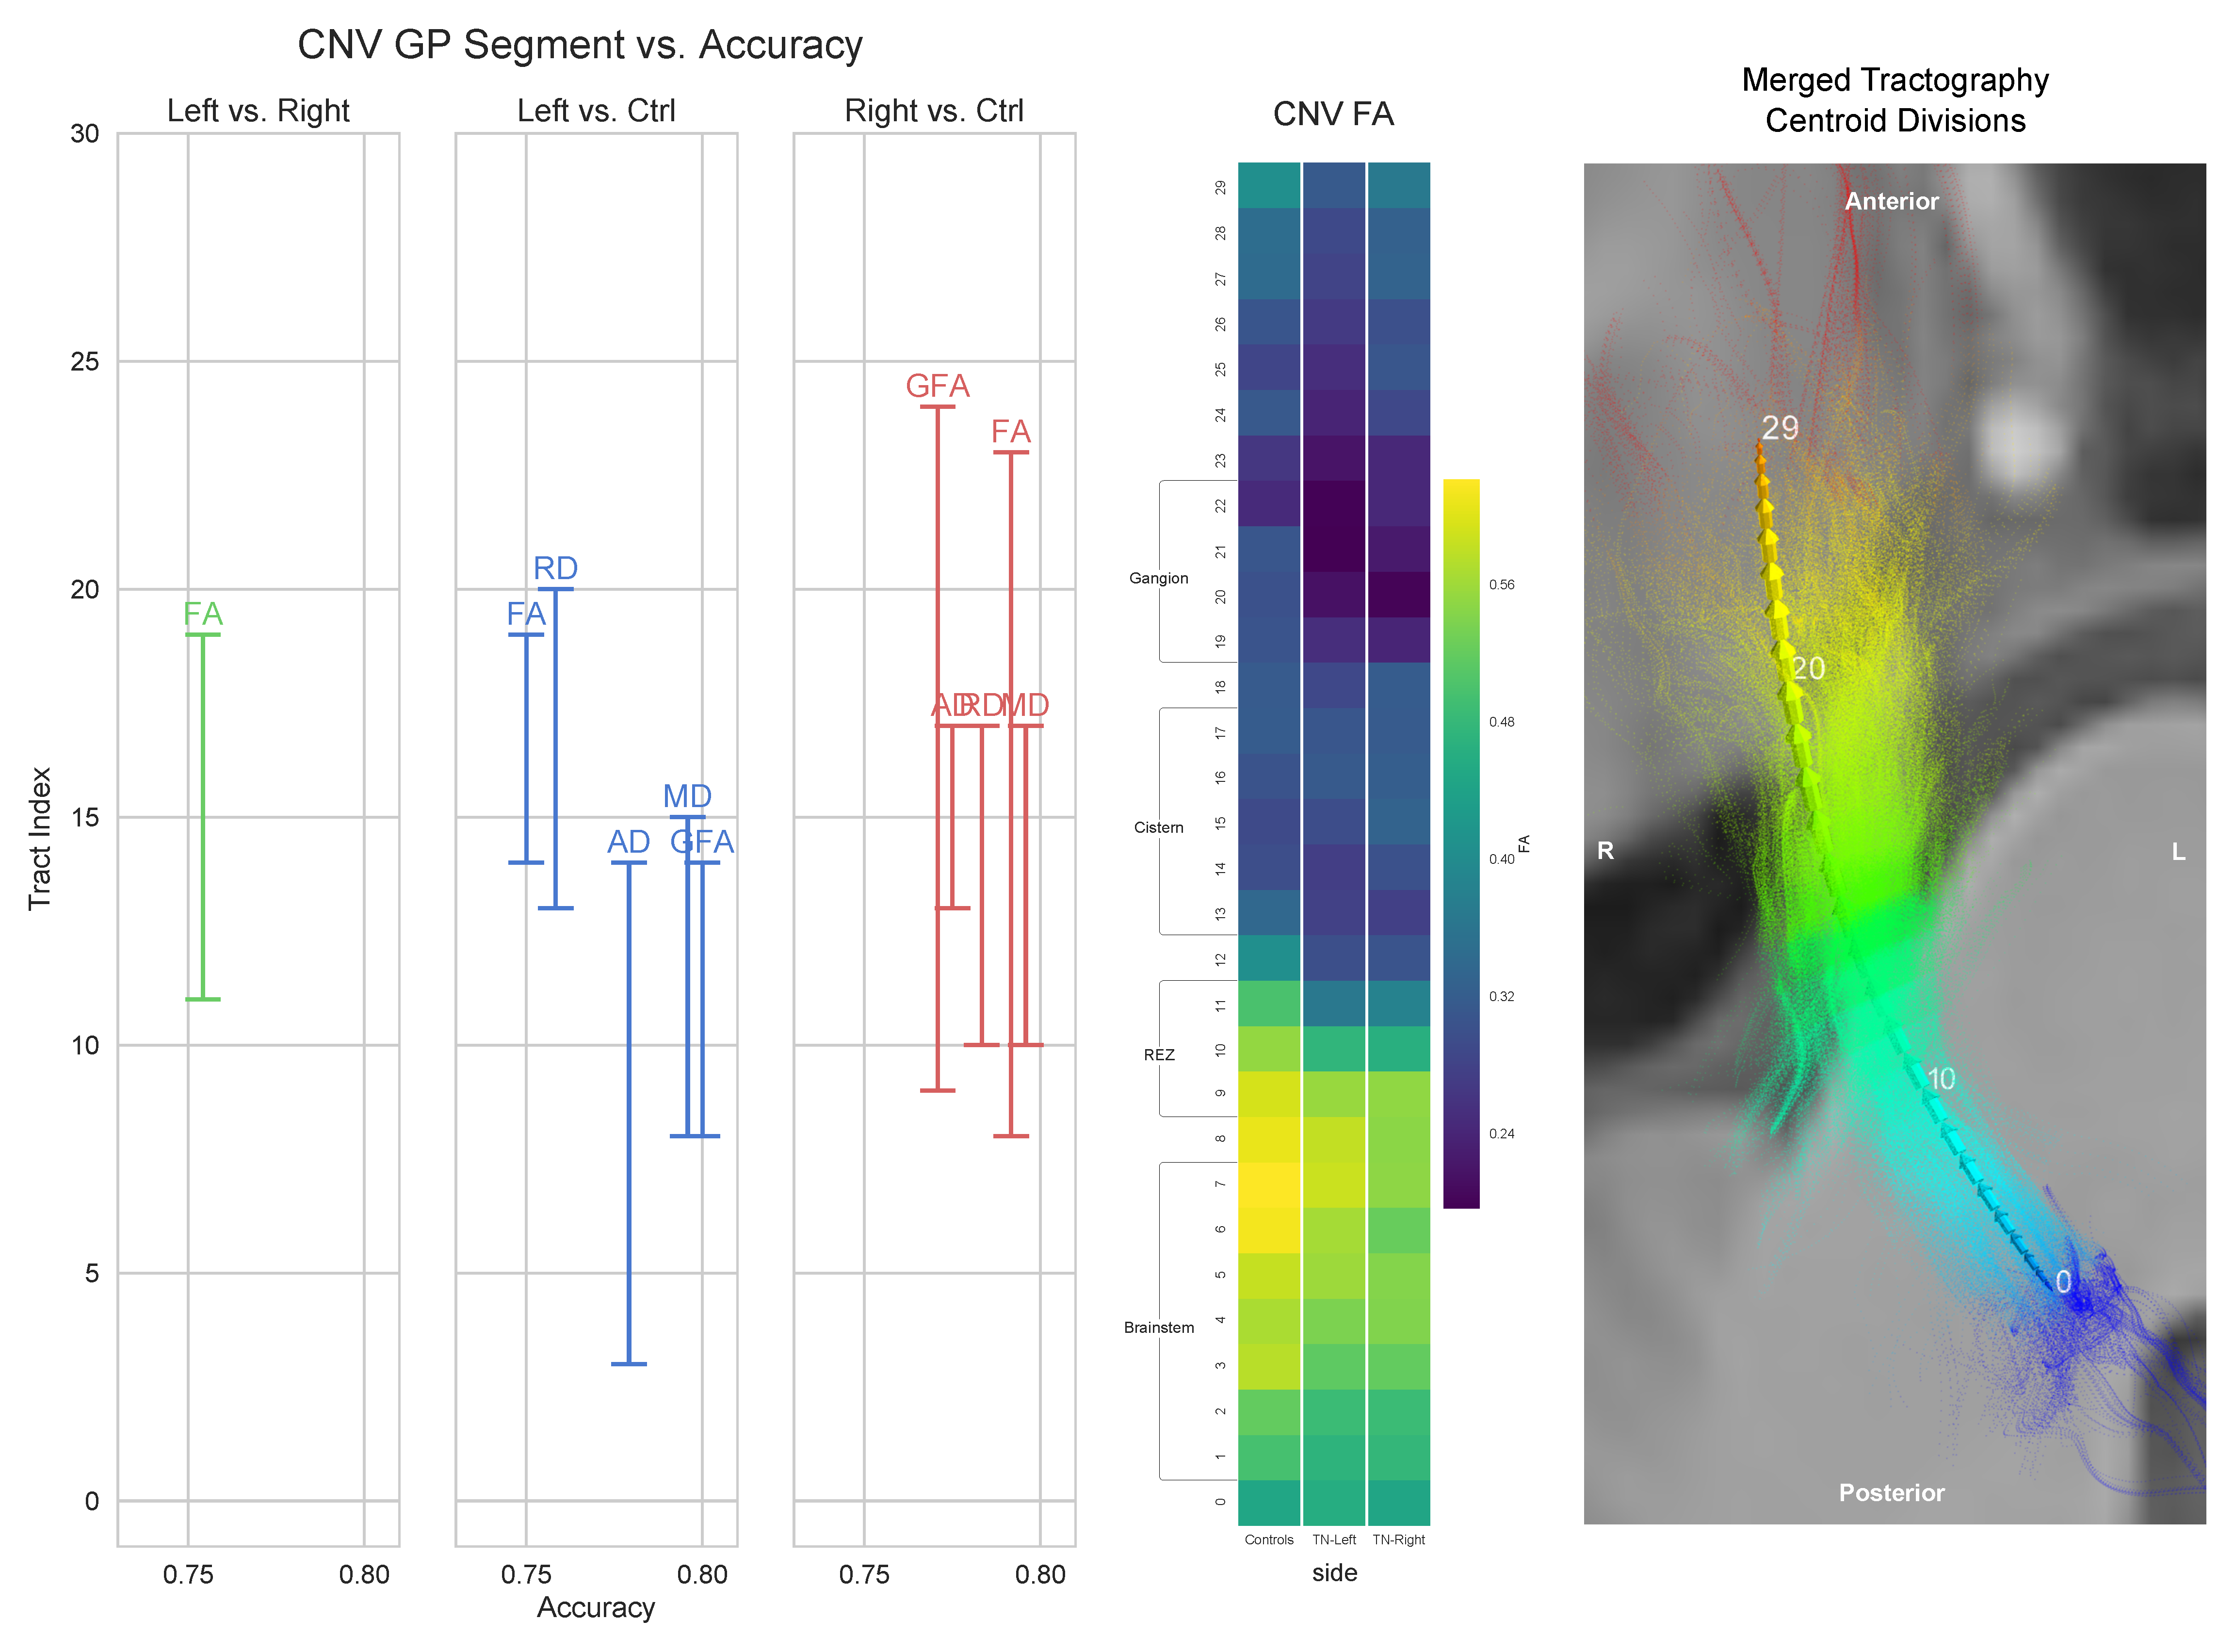
\includegraphics[width=1.2\textwidth,center]{figure-GP-CNV.pdf}
\caption{CN V classifier performances. This figure consists of 3 panels. Panel A, y axis represents the anatomical subregions of the trigeminal nerve as defined by the centroid subdivisions (see Figure \ref{fig:GPfigure-method-centroid}). Panel A, x-axis denotes the accuracy of the classifiers (scale of 0-1, with 1 representing 100\%)). Each diffusivity is denoted with respect to the window size (see Figure \ref{fig:GPfigure-method-centroid}) and position along the centroid where the accuracy is derived from. 3 instances are studied: comparison of left (unaffected) vs. control (average of both trigeminal nerves), comparison of right (affected) vs. control and comparison of left (unaffected) vs. right (affected). The colours for the diffusivity in each panel in A is arbitrary. Panel B is a heatmap (raw visualization) of FA values of the corresponding centroid positions. Panel C shows the centroid and point assignments for anatomical reference. The colours of the points correspond to their respective subdivision position as described in figure \ref{fig:GPfigure-method-centroid} and figure \ref{fig:GPfigure-method-centroid}} throughout the figure, the position of the centroid subdivisions are aligned and expressed with respect to the anatomical position as per panel B.
\label{fig:GPfigure4}
\end{figure}

\paragraph{Trigeminopontothalamic tract}
Classifiers could distinguish bilateral TPT pathways (affected and unaffected) from controls with greater than 80\% accuracy (Figure \ref{fig:GPfigureTPT}). The right (affected) FA classifier achieved the greatest accuracy at 85\% versus controls, and right RD classifier was least accuracy at 83\%. The left (unaffected) FA classifier showed greatest accuracy at 89\% and left RD classifier showed the least accuracy at 71\%. The classifiers covered both the decussation and the ascending segments of the TPT, with the right decussation showing more proximal coverage. The left-versus-right classifiers achieved maximum accuracy of 98\% (FA) and minimum of 88\% (MD). The FA classifier covered position 4--14, suggesting strong laterality differences in the TPT (Table \ref{table:GP}). 

\begin{figure}[ht]
\centering
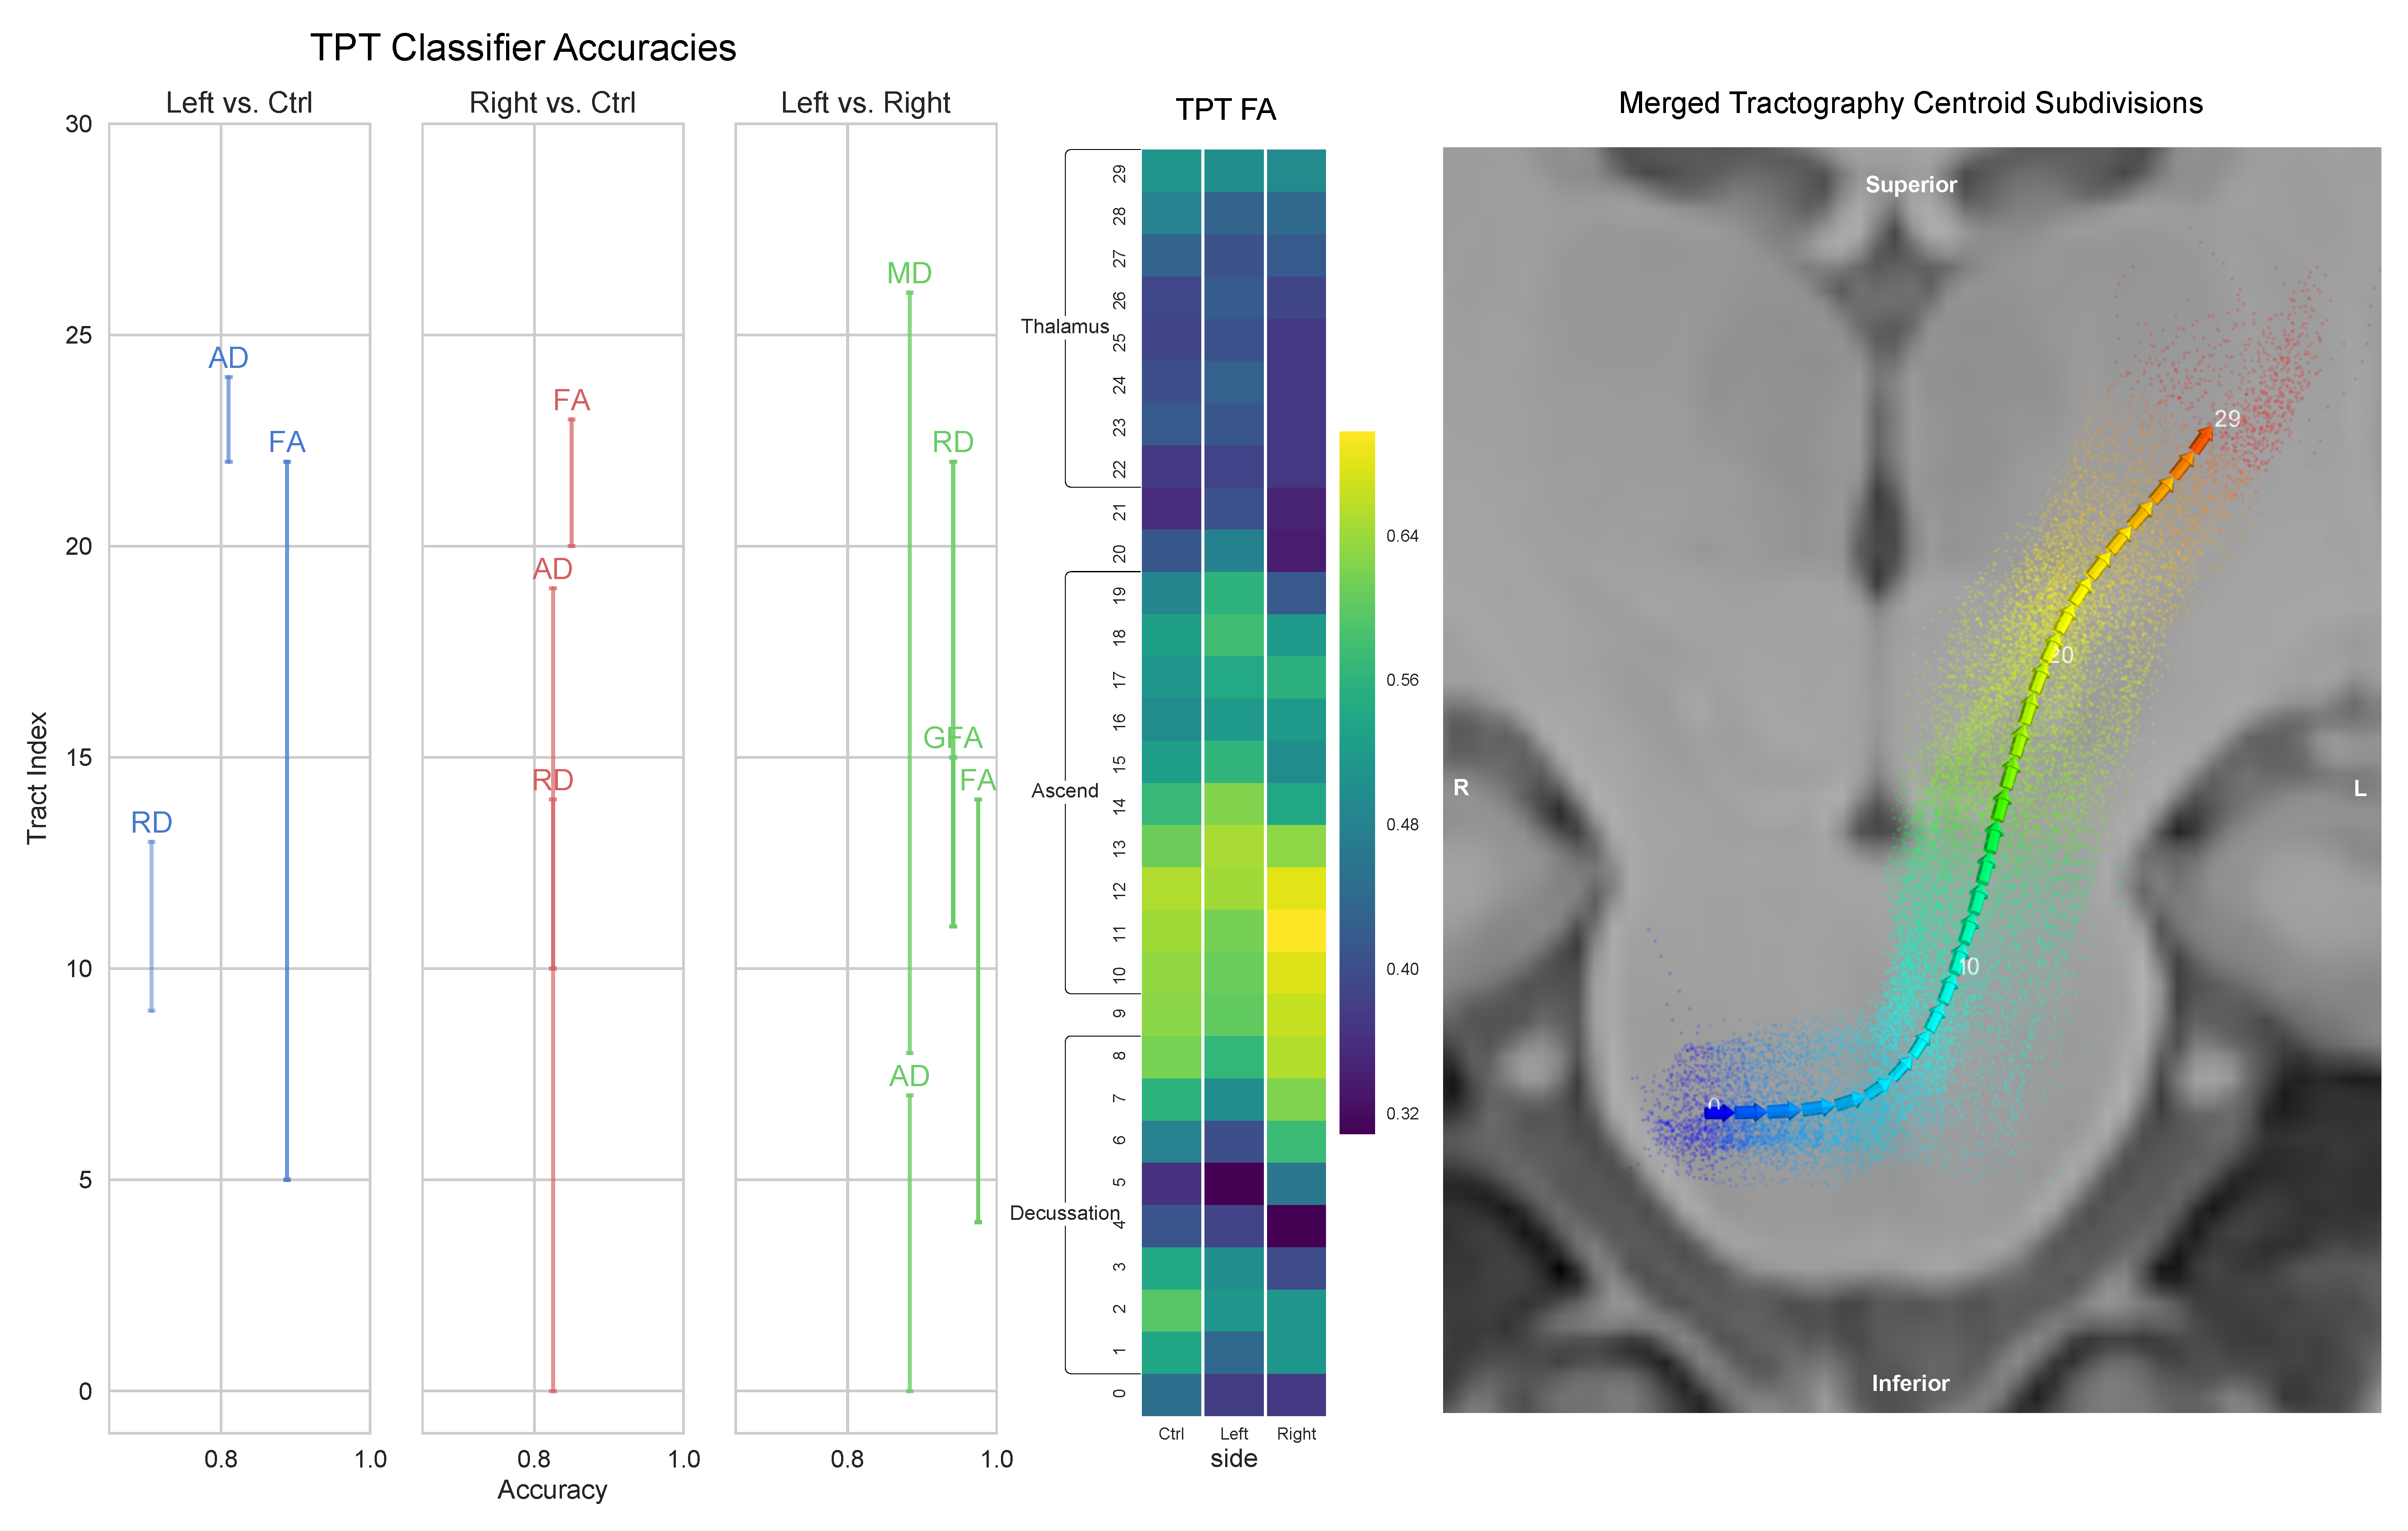
\includegraphics[width=1.2\textwidth,center]{figure-GP-TPT.pdf}
\caption{TPT classifier performance, see Figure \ref{fig:GPfigure4} for details on annotations.}
\label{fig:GPfigureTPT}
\end{figure}

\paragraph{S1}
Classifiers distinguished bilateral S1 face region pathways from controls with 85\% accuracy. The left (affected) RD classifier achieved maximal accuracy of 87\% at position 13--20, while the right (unaffected) RD classifier achieved maximal accuracy of 83\% at position 8--26 (Figure \ref{fig:GPfigure5}). Overall the left classifier ranged from 72\% (AD) to 87\% (RD), and the right classifiers ranged from 73\% (GFA) to 83\% (RD) (Table \ref{table:GP}). Classifiers of both sides covered the the branching region between the thalamus and cortex. Left-versus-right classifiers showed maximum accuracy of 78\% (RD), and minimum of 76\% (FA). The left-versus-right classifiers overlap in the regions 5--10, at the segment where the pathway emerges from the thalamus.

\begin{figure}[ht]
\centering
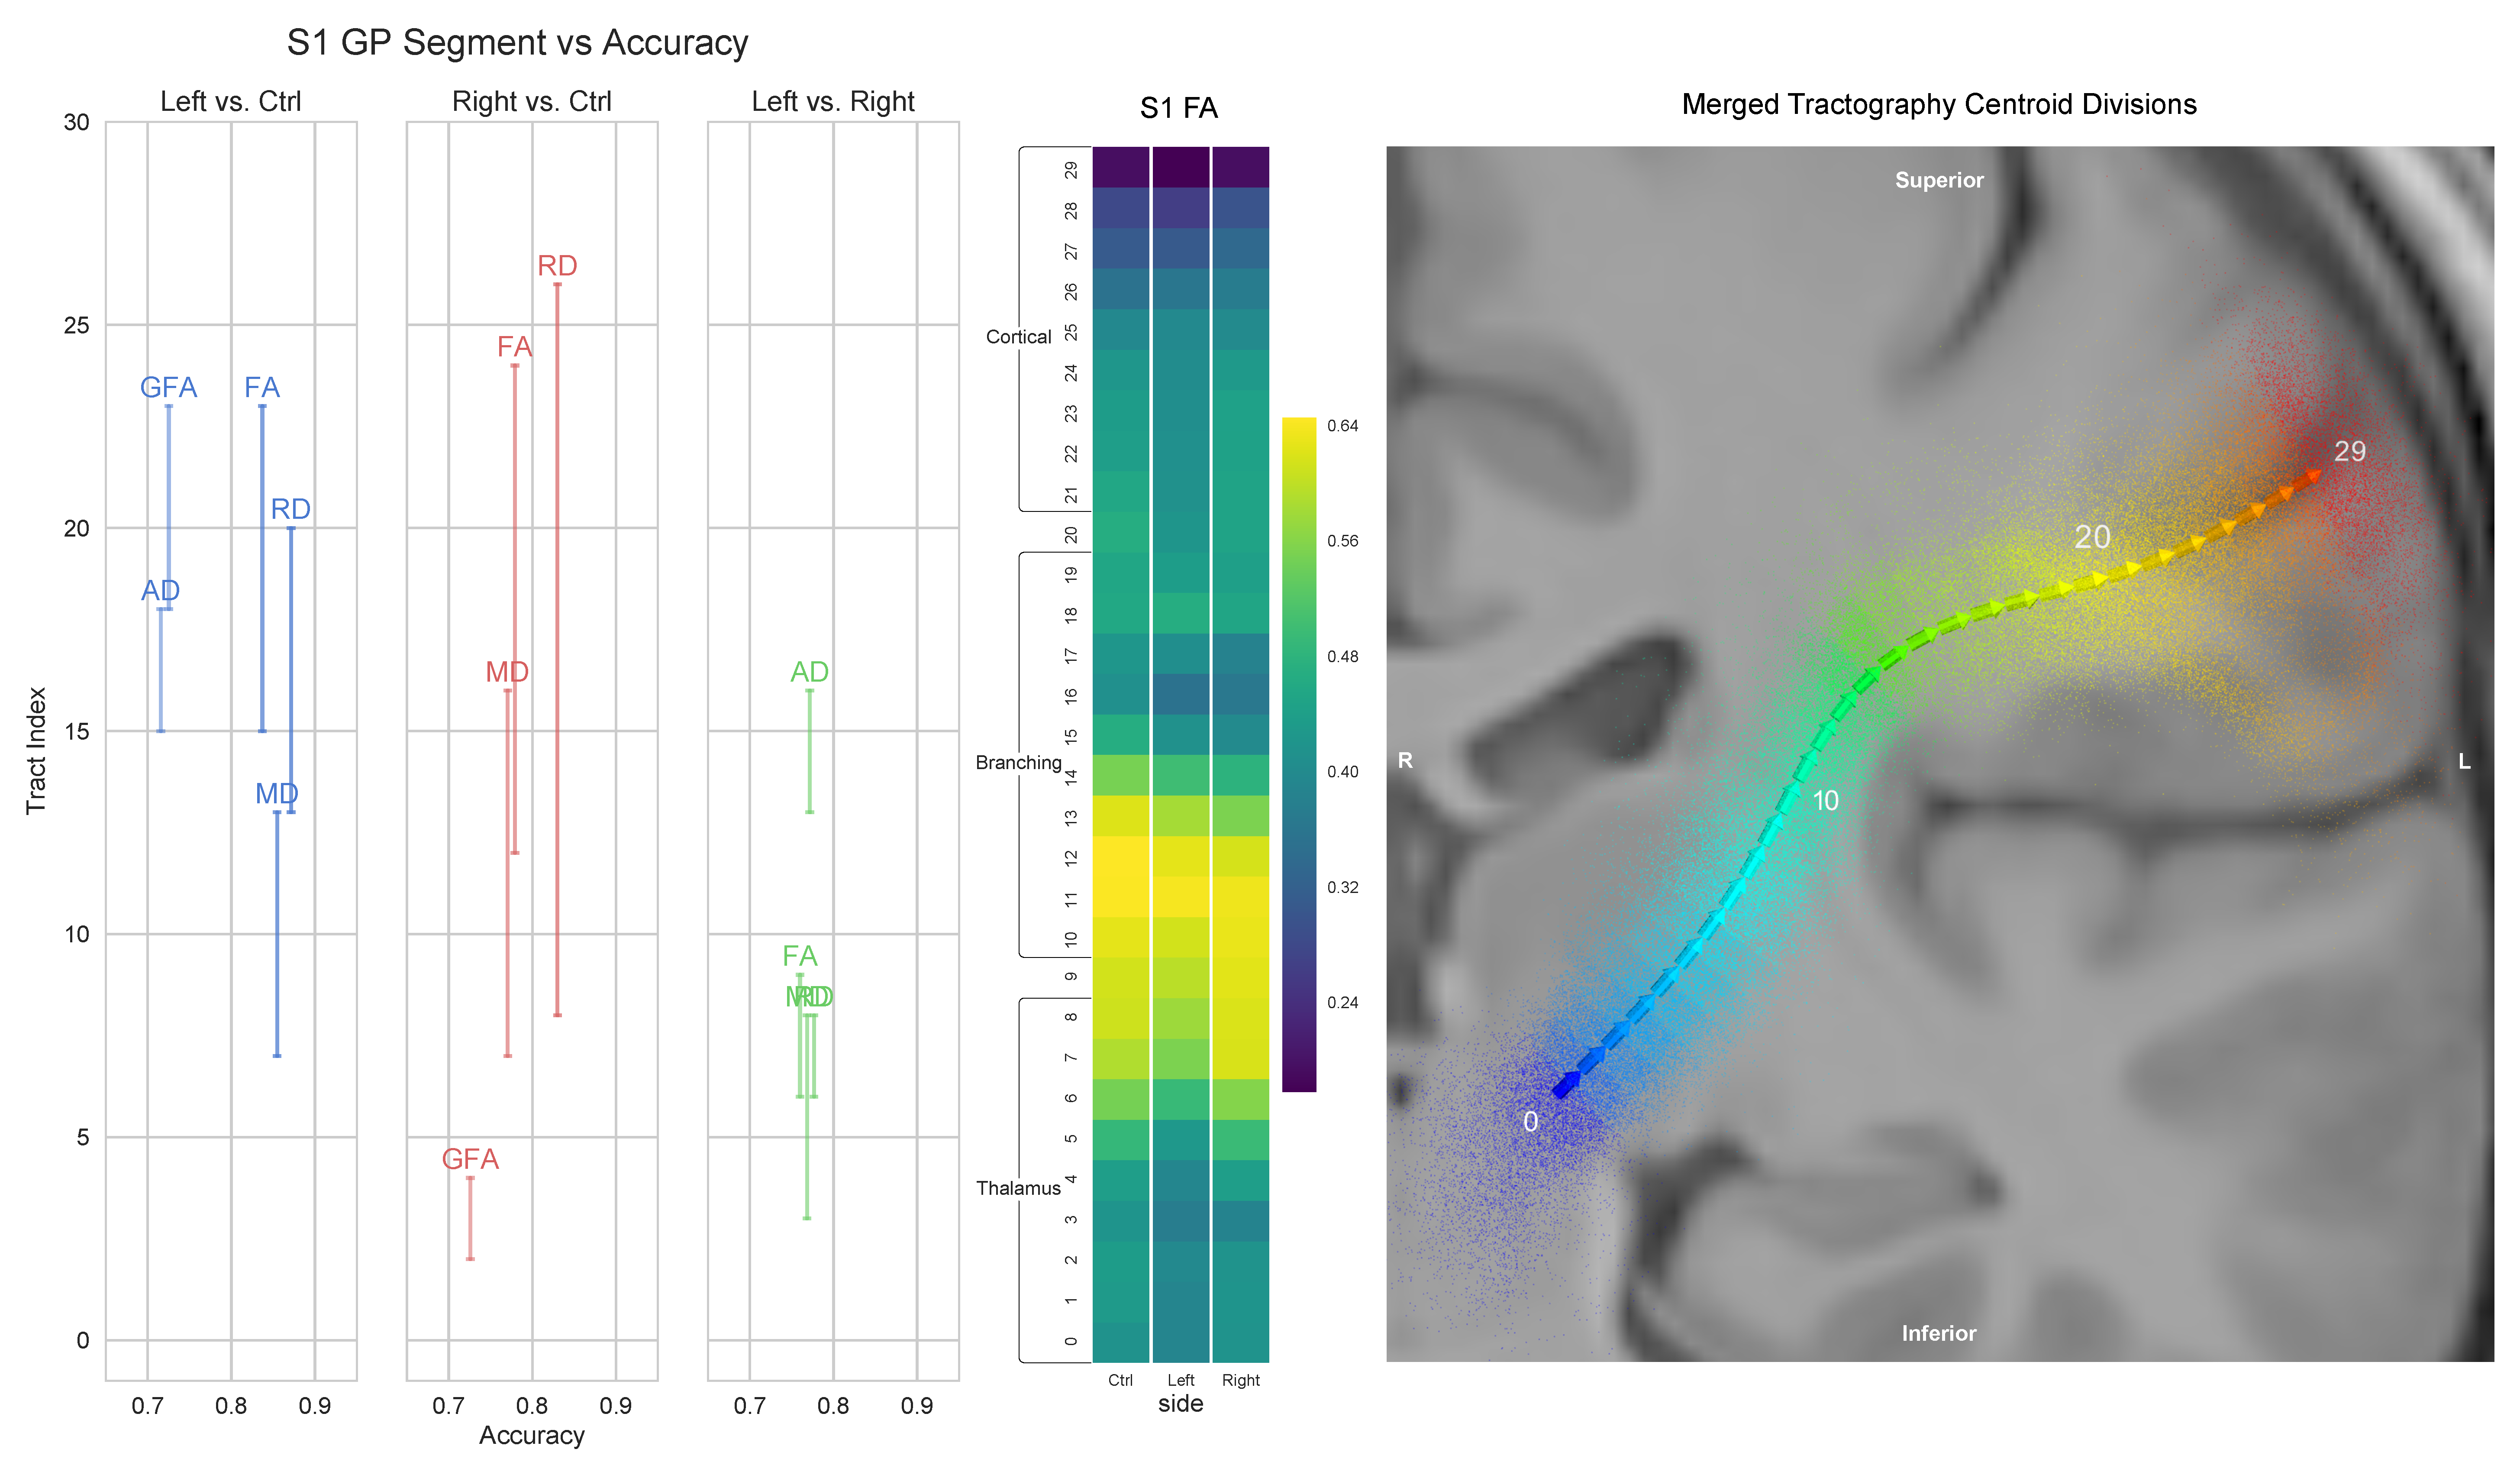
\includegraphics[width=1.2\textwidth,center]{figure-GP-S1.pdf}
\caption{S1 classifier performance, see Figure \ref{fig:GPfigure4} for details on annotations.}
\label{fig:GPfigure5}
\end{figure}

\begin{table}[p]
\centering
\small
\csvautotabular{tn_sagit_table.csv}
\caption{List of the best GP models for different diffusivity metrics and centroid windows. Only models with at least 70\% accuracy were accepted. Table is sorted by anatomical region, classifier type (R denotes right (affected) side versus controls; L denotes left (unaffected) side versus controls; LVR denotes left-versus-right ) and accuracy. Start and end denote the beginning and end of the window subdivision positions along the centroid. Length is the number of subdivisions covered by the window. Precision and f1 scores are provided for reference}
\label{table:GP}
\end{table}

\section{Discussion}
We have demonstrated the use of a fully-automated, end-to-end tractography and machine learning platform that is capable of discriminate TN from white-matter diffusivity with greater than 80\% accuracy strictly from white-matter measures. Our work is in agreement with previous findings of TN diffusivity changes along the CN V, yet the present technique offers much higher regional specificity, as well as examining the TPT and S1 projections of the trigeminal sensory pathway. The study is the first instance of machine learning discrimination of TN vs. controls with specific white matter analysis, using group-wise merged along-the-track tractography. 

The diffusivity measures of CN V agreed with our previous findings \cite{Chen2016a}, that the cistern, REZ differentiated TN from controls. The consistent regional overlaps in the cistern/ganglion region of the right (affected) CN V showed the ability for the GP classifiers to auto-converge to focal white-matter abnormality. The GP classifier placed affected vs unaffected differences at the cistern/REZ segment, in agreement with the pathophysiology of focal neurovascular compression in TN. 

The findings on unaffected (left) versus controls suggests bilateral differences in CN V diffusivities in unilateral TN, despite the lack of symptoms on the unaffected side. RD and AD have previously shown to relate to myelination \cite{Song2002} and axonal integrity \cite{Budde2009}. Therefore this finding is significant, since it suggests that the REZ and brainstem CN V ultrastructure might be bilaterally affected in unilateral TN pain, a process that may play important role in TN pain chronification, and responsiveness to surgery. The classifier windows of unaffected side also situate into the brainstem subdivisions. It is possible that the unaffected CN V is modulated by descending pathways \cite{Davis2013,Bushnell2013}. This point warrants further investigation.

The TPT left-verus-right FA/RD/GFA classifiers demonstrated very high accuracy (\textgreater 90\%), with overlapping windows in the ascending segment. The TPT merged tractography delineations showed that decussation pathway tractography is possibly asymmetric. The asymmetry of this decussation has not been demonstrated before. It is not clear whether this represents the anatomical arrangement of these fibers, or whether decussations are always purely symmetrical (akin to a perfectly shuffled deck of cards). Further assessment of other decussation points will be helpful to understand this process.  

We were able to successfully delineate the course of the fibers from the thalamus to S1 given the use of SAGIT and incorporation of Freesurfer cortical segmentation maps. Previous studies have suggested that S1 is involvement in pain location discrimination \cite{bushnell1999pain}, and have been found to exhibit grey-matter abnormalities in TN pain \cite{Desouza2013c}. We found that that while the left (affected) S1 RD classifier had higher accuracy (87\%) compare to the right S1 RD classifier (83\%), the left-verus-right classifier windows showed more overlap in subdivisions close to the thalamus. This suggests that while there is bilateral difference in the S1 pathways from controls, the difference between the segments mitigates as these reach closer to the S1 cortex.


The classifier windows showed a large variation of size. For example, amongst CN V classifiers (Figure \ref{fig:GPfigure3}), right MD consisted of 18 subdivisions, while right FA consisted of 7; The left classifiers showed a variety of sizes, yet the accuracy derived from each classifier were near 80\%. In the same manner, we observed variabilities in TPT and S1 classifiers window sizes. This suggests that classification according to a single diffusivity metric may be difficult to interpret, and thus multiple metric classifiers should be considered together. 

FA classifiers consistently achieved the highest accuracy in CNV and TPT, with the exception of S1. This might be due to the fact that it is known to have trouble in regions of heavy crossing-fibers. However, the TPT pathway also situations in regions of complex crossing fibers. One explanation for FA classifier in TPT is that the pathway courses through the narrow passage of pontine/thalamic regions, the fiber structures are highly constrained. Therefore FA still remains as a sensitive diffusivity metric for the TPT. 

We included GFA to investigate its potential for measuring cross-fiber white-matter diffusivity, as it is the most well-known non-Gaussian diffusivity metric. Although metrics such as FA are popular in current neuroimaging literature, they nevertheless are derived from the Gaussian tensor model, which cannot adequately describe cross-fiber regional dynamics. For example, in the crossing-fiber region of healthy tissue, where both bundles have equal myelin and axonal integrity, will have a low FA score due to a spherical tensor; its AD and RD will be roughly equal, and therefore MD will be higher. In a pathological cross region, where only one bundle is healthy, the FA increases due to the diffusivity bias in one direction; the RD will be lower, and MD will be lower as well. Moreover, in diverging and converging structures, as well as in multi-crossing regions such as the corona radiata, the interpretations of Gaussian-based diffusivity metrics become even more unclear. However results demonstrated that GFA did not perform to any substantially degree than the Gaussian-based diffusivity metrics such as FA. 

Overall the GP classifiers windows revealed areas in the TN pathways that would not have been captured using singular diffusivity metric analysis. Cross-metric features therefore should be considered in future studies. 

\subsubsection{Limitations}
The merged CN V delineations of all the subjects showed caudal projections towards the spinal cord. The consistent observation of diverging streamlines at the levels of the medulla strongly suggests that these fibers correspond to trigeminal spinal decussations. However the caudal projection were not consistently seen. This is likely due to the limited size of voxel resolution that in turn does not permit adequate resolution of medullary and spinal cord fiber details.

The DWI images were acquired at 0.9375$\times$0.9375$\times$3 $mm\textsuperscript{3}$ voxel resolution. The acquisition was a compromise to allow better in-plane resolution to image the trigeminal nerve, due to the limits of the 3T GE HDx MRI with 8-channels head coil. Our analysis is internally consistent, and SAGIT was previously validated on a identical sequence \cite{Chen2016,Chen2016a}, highlighting the validity of this approach. 

\subsection{Conclusions}
We have demonstrated group-wise along-the-track tractography machine learning analysis of TN vs. control. We have achieved the examination of specific and targeted anatomy at a group level involving both healthy and pathological brain images. The method agreed with previous findings of TN diffusivity changes along the CN V with finer-grained regional specificity. We also examined TPT and S1 projections of the trigeminal sensory pathway. The study revealed that there are specific diffusivity changes on these deeper white matter structures, and demonstrated the power of along-the-tract analysis with machine-learning, which pinpoints the exact location of the diffusivity disruption at millimetre level. 
